\documentclass[12pt]{amsart}
\usepackage{a4}
\usepackage{amsmath,amssymb,amsthm}
\usepackage{multicol}
\usepackage{verbatim}
\usepackage{graphicx}
\newcommand{\sgn}{\mathop{\mathrm{sgn}}}
\newcommand{\ignore}[1]{}
\newcommand{\mat}[4]{\left(\begin{array}{ccc} #1 & #2 \\#3 & #4 \end{array} \right)}
\newcommand{\vect}[2]{\left(\begin{array}{ccc} #1 \\#2 \end{array} \right)}
\newcommand{\matc}[9]{\left(\begin{array}{ccc} #1 & #2 & #3 \\#4 & #5 & #6 \\#7 & #8 & #9 \end{array} \right)}
%\newcommand{\matd}[16]{\left(\begin{array}{ccc} #1 & #2 & #3 & #4 \\#5 & #6 & #7 & #8 \\#9 & #10 & #11 & #12 \\#13 & #14 & #15 & #16 \end{array} \right)}
\begin{document}

%It's simple to make manifolds of constant curvature

In order to allow more interesting manifolds than a few that I hard code in, I plan to implement connected sums of manifolds. Unfortunately, almost none of the well-known manifolds can be smoothly connected without changing their metrics. In order to facilitate this, I have found a class of manifolds that can be used as intermediates to smoothly connect two manifolds of constant curvature, and which allows geodesics to be easily calculated. I call them wormholes.

\begin{figure}

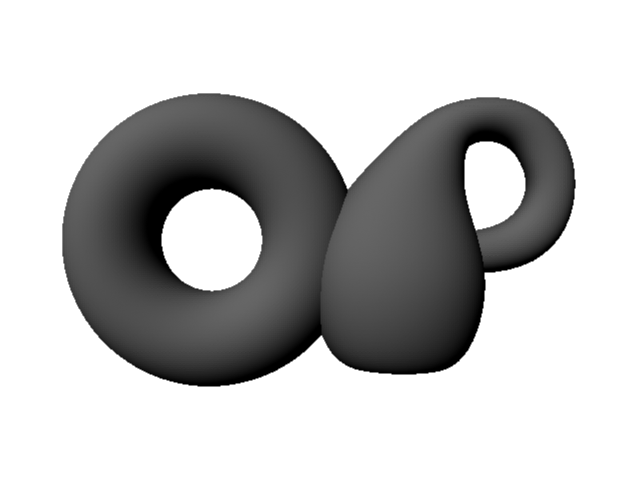
\includegraphics[scale=0.3]{../slideshow/IntersectingSpaces.png}

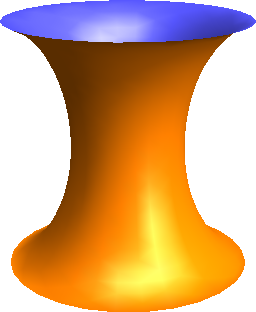
\includegraphics[scale=0.3]{PortalSpace.png}

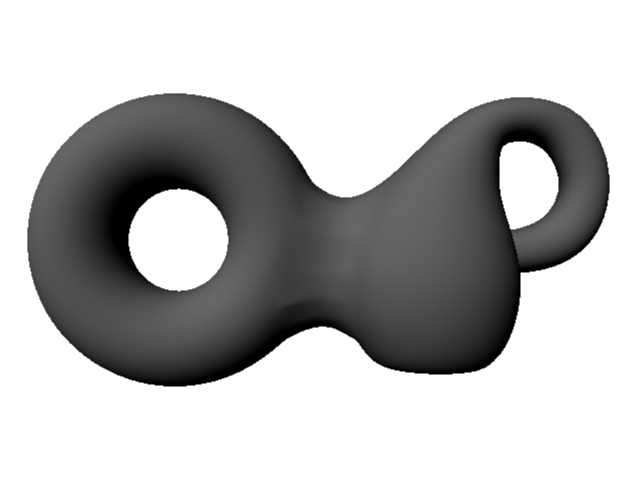
\includegraphics[scale=0.3]{../slideshow/MergedSpaces.png}

\end{figure}

???

%Let an $n$-lathe be the surface made by spinning a curve along an $n-1$-sphere.

%Consider a geodesic on a $3$-surface of revolution made by rotation a curve along a sphere.

Consider a point $x$ on a $3$-surface $U$ of revolution made by rotating a curve along a sphere, and a vector $v$ in the tangent space $U_x$.

Consider the component $v_0$ of $v$ along $S^2$.

Consider the great circle made by extending $x$ to a geodesic in the direction of $v_0$.

We can reflect across this great circle on all the spherical cross-sections of $U$.

By symmetry, the geodesic made by extending $x$ in the $v$ direction must stay on this slice of $U$.

This reduces finding the geodesic on a $3$-surface of revolution to finding one on a $2$-surface.

Consider the quotient space in $\mathbb{H}^2$ made by identifying two ultraparallel lines so that the intersections with their mutual perpendiculars are identified, and they both go in the same direction.

Then a miracle happend.

The resulting space is a surface of revolution.

We can extend this to a $3$-surface of revolution, then use the above method to reduce finding a geodesic to finding one on this space.

???

$y_0 = a\sin(x_0-\theta_0), y_1 = a\sin(x_1-\theta_0)$

$\frac{y_1}{y_0} = \frac{\sin(x_1-\theta_0)}{\sin(x_0-\theta_0)}$

???

Rather than mapping a sphere to $\mathbb{R}^2$, we can embed it in $\mathbb{R}^3$.

Given points $\textbf{x}, \textbf{y}$,

First, we take the first thee coordinates, which gives us points in $S^2$.

We can easily find the great circle between them.

We set up a geodesic along $\mathbb{H}^2$, and place $\textbf{x}$ at the distance given by $x_4$ from the bottleneck, where the spherical cross-section is thinnest.

We then move along the spherical cross-section a distance equal to the distance the first three coordinates of $\textbf{x}$ are along the great circle. We do this simply by scaling $e^{k\theta}$, where $\theta$ is the angle along the great circle, and $k$ is some constant that depends on the specific surface we're using.

%The curvature along the bottleneck will be $\frac{1}{k}$.???

We do a similar process for $\textbf{y}$.

Now we can find the geodesic between them along this $\mathbb{H}^2$ slice.

We can then find the vector representing the distance and direction from $\textbf{x}$ to $\textbf{y}$.

Now we simply transform this back to a point on the full space.

$(v_1,v_2,v_3)$ is the component of $\textbf{v}$ along the $S^2$ slice, which is just the the component along the line perpendicular to the circle on the euclidean map used to represent the hyperbolic slice. Just transform this back onto $S^2$. Don't worry about the radius of $S^2$. We didn't actually use it to calculate distance, so it doesn't matter.

$v_4$ is the component of $\textbf{v}$ orthogonal to the $S^2$ slice, which is along the cricle on the euclidean map of the hyperbolic slice.

\ignore{
%This won't work.
There is one more problem. There are multiple images of $\textbf{y}$ from $\textbf{x}$. They are all just multiples of $e^{2\pi k}$, but the problem is connecting them to the correct other images in a triangle. In order to do that, I need to standardize which is being referred to.

When finding the great circle on $S^2$, we need to find where it intersects with some imaginary line. For example, $z_2 = 0, z_1 \geq 0$.

The equation for the great circle is $\textbf{x}\cos\theta + \textbf{y}'\sin\theta$. Thus, we have to find $x_2\cos\theta + y'_2\sin\theta = 0$

$\frac{x_3}{y'_3} = \tan\theta$

$\theta = \arctan\frac{x_3}{y'_3}$

Only every other value for that is correct. We just have to test to see if the first attempt fulfills $x_1\cos\theta + y_1\sin\theta \geq 0$, and add $\pi$ if it does not.

Now we add or subtract $2\pi$ to make sure it's in the correct range.

We make sure to store an extra integer $n$ in $\textbf{y}$, representing how many extra loops around the circle it goes. Once we move it into the $\mathbb{H}^2$ slice, we just multiply it by $e^{nk}$ to make sure it's in the right place.

The purpose of this is that I need a covering map that shows how many loops around it went. In this case, I used the universal covering space of $S^2$ minus the poles. I essentially did it on a nonstandard topology of $S^2 \times \mathbb{Z}$.
}

\bigskip

Now to find the geodesic from the vector.

\bigskip

First, we look at this on the $\mathbb{H}^2$ slice.

We move $x$ onto $\mathbb{H}^2$ by letting the angle on the geodesic represented by a circle about the origin be $x_4$. The radius doesn't matter for this, since it doesn't matter where we start the section of the quotient space we look at. Thus, we can map it to $\textbf{x}' = (\sin x_4,\cos x_4)$.

$v_4$ gets mapped perpendicular to the direction of $\textbf{x}'$ from the origin on the Euclidean plane. The rest of $\textbf{v}$ gets pointed along it.

Now that we have a vector in $\mathbb{H}^2$, we can construct the geosic as when we did it in a slice of $\mathbb{H}^3$.

Once we have $\textbf{y}'$, we let $y_4 = \arctan\frac{y'_1}{y'_0}$.

$e^{k\theta} = \|\textbf{y}'\|$

$\theta = \frac{1}{k}\ln\|\textbf{y}'\|$

$= \frac{1}{2k}\ln\|\textbf{y}'\|^2$

$(y_1,y_2,y_3) = (x_1,x_2,x_3)\cos\theta + (v_1,v_2,v_3)\sin\theta$

Finding the rotation is more difficult.

First, consider the two-dimensional rotation.

???

%Let $\textbf{x}'' = \frac{\textbf{x}'}{|\textbf{x}|}, \textbf{y}'' = \frac{\textbf{y}'}{|\textbf{y}'|}$.

$\sin\theta_0 = \frac{\textbf{x}' \times (\textbf{x}'-\textbf{c})}{|\textbf{x}'||\textbf{x}'-\textbf{c}|}$

$= \frac{x'_0(x'_1-c_1) - x'_1(x'_0-c_0)}{\sqrt{|\textbf{x}'|^2|\textbf{x}'-\textbf{c}|^2}}$

$= \frac{x'_0 x'_1 - x'_1(x'_0-c_0)}{\sqrt{|\textbf{x}'|^2|\textbf{x}'-\textbf{c}|^2}}$

$= \frac{c_0 x'_0}{\sqrt{|\textbf{x}'|^2|\textbf{x}'-\textbf{c}|^2}}$

$\cos\theta_0 = \frac{\left<\textbf{x}',\textbf{x}'-\textbf{c}\right>}{|\textbf{x}'||\textbf{x}'-\textbf{c}|}$

$\sin\theta_1 = \frac{\textbf{y}' \times (\textbf{y}'-\textbf{c})}{|\textbf{y}'||\textbf{y}'-\textbf{c}|}$

$= \frac{c_0 y'_0}{\sqrt{|\textbf{y}'|^2|\textbf{y}'-\textbf{c}|^2}}$

$\cos\theta_1 = \frac{\left<\textbf{y}',\textbf{y}'-\textbf{c}\right>}{|\textbf{y}'||\textbf{y}'-\textbf{c}|}$

$\mat{\cos\theta_1}{-\sin\theta_1}{\sin\theta_1}{\cos\theta_1}\mat{\cos\theta_0}{\sin\theta_0}{-\sin\theta_0}{\cos\theta_0}$

Let $\textbf{z} =$ the normalization of the component of $\textbf{y}$ perpendicular to $\textbf{x}$.

I'm going to need to commute this with a matrix that moves $\textbf{z}$ to $(0,1,0,0)$. I'm going to make the first digit be the distance along the arc in $\mathbb{H}^2$.

Let's just let it move $\textbf{x}$ to $(0,0,1,0)$ and $\textbf{x} \times \textbf{z}$ to $(0,0,0,1)$. It will preserve $(1,0,0,0)$.

This makes the matrix

???

$\textbf{e}_1 \mapsto \textbf{e}_1, \textbf{z} \mapsto \textbf{e}_2, \textbf{x} \mapsto \textbf{e}_3, \textbf{x} \times \textbf{z} \mapsto \textbf{e}_4$

$(\textbf{e}_1, \textbf{z},\textbf{x},(\textbf{x} \times \textbf{y}'))^{-1}$

$= (\textbf{e}_1, \textbf{z},\textbf{x},(\textbf{x} \times \textbf{y}'))^T$, since it's a rotation matrix.

???

$(\textbf{e}_1,\textbf{z},\textbf{x},(\textbf{x} \times \textbf{z}))^T$

$$(\textbf{e}_1,\textbf{z},\textbf{x},(\textbf{x} \times \textbf{z}))
\left(\begin{array}{cccc} \cos\theta_1 & -\sin\theta_1 & 0 & 0 \\ \sin\theta_1 & \cos\theta_1 & 0 & 0 \\ 0 & 0 & 1 & 0 \\ 0 & 0 & 0 & 1 \end{array} \right)
\left(\begin{array}{cccc} \cos\theta_0 & \sin\theta_0 & 0 & 0 \\ -\sin\theta_0 & \cos\theta_0 & 0 & 0 \\ 0 & 0 & 1 & 0 \\ 0 & 0 & 0 & 1 \end{array} \right)
(\textbf{e}_1,\textbf{z},\textbf{x},(\textbf{x} \times \textbf{z}))^T$$

This still fails to take into account the rotation around the sphere.

It just rotates between $\textbf{x}$ and $\textbf{z}$, so if we do it mid-conjugation, we can just do it with a $2 \times 2$ matrix like so:

$$(\textbf{e}_1,\textbf{z},\textbf{x},(\textbf{x} \times \textbf{z}))
\left(\begin{array}{cccc} 1 & 0 & 0 & 0 \\ 0 & \cos\theta & -\sin\theta & 0 \\ 0 & \sin\theta & \cos\theta & 0 \\ 0 & 0 & 0 & 1 \end{array} \right)
\left(\begin{array}{cccc} \cos\theta_1 & -\sin\theta_1 & 0 & 0 \\ \sin\theta_1 & \cos\theta_1 & 0 & 0 \\ 0 & 0 & 1 & 0 \\ 0 & 0 & 0 & 1 \end{array} \right)$$ $$
\left(\begin{array}{cccc} \cos\theta_0 & \sin\theta_0 & 0 & 0 \\ -\sin\theta_0 & \cos\theta_0 & 0 & 0 \\ 0 & 0 & 1 & 0 \\ 0 & 0 & 0 & 1 \end{array} \right)
(\textbf{e}_1,\textbf{z},\textbf{x},(\textbf{x} \times \textbf{z}))^T$$

Where $\theta = \frac{1}{2k}\ln\|\textbf{y}'\|^2$

\ignore{

We can reflect across great circles on $S^2$, and show by symmetry that the geodesic must pass through $S^1 \times \mathbb{R}$.

Now, consider the case of a geodesic on a $2$-surface of revolution.

Let $f(x)$ be the function on the surface of revolution.

???

Consider the metric on $S^2 \times \mathbb{R}$

???

$ds^2 = vdu^2+f(v)dv^2$

???

$h_u = f(v), h_v = 1$

$E = f^2(v), F = 0, G = 1$

$E_v = 2f(v)f'(v)$

$E_u = G_u = G_v = 0$

$\Gamma^1_{11} = \Gamma^1_{22} = \Gamma^2_{12} = \Gamma^2_{22} = 0$

$\Gamma^1_{12} = \frac{E_v}{2E}$

$= \frac{2f(v)f'(v)}{2f^2(v)}$

$= \frac{f'(v)}{f(v)}$

$\Gamma^2_{11} = -\frac{E_v}{2G}$

$= -f(v)f'(v)$

$0 = \kappa_g = \sqrt{EG-F^2}[-\Gamma^2_{11}{u'}^3+\Gamma^1_{22}{v'}^3-(2\Gamma^2_{12}-\Gamma^1_{11}){u'}^2v'+(2\Gamma^1_{12}-\Gamma^2_{22})u'{v'}^2+u''v'-v''u'] \times (E{u'}^2+2Fu'v'+G{v'}^2)^{-3/2}$

$= |f(v)|[f(v)f'(v){u'}^3+2\frac{f'(v)}{f(v)}u'{v'}^2+u''v'-v''u'] \times (f^2(v){u'}^2+{v'}^2)^{-3/2}$

Since it will work out as the same manifold if part or all of it is inside out, we can assume WLOG $f(v) \geq 0$

$\kappa_g = f(v)[f(v)f'(v){u'}^3+2\frac{f'(v)}{f(v)}u'{v'}^2+u''v'-v''u'] \times (f^2(v){u'}^2+{v'}^2)^{-3/2}$

Since we're only interested in $\kappa_g = 0$,

$f(v)f'(v){u'}^3+2\frac{f'(v)}{f(v)}u'{v'}^2+u''v'-v''u' = 0$

Assume WLOG $u' = 1$

$f(v)f'(v)+2\frac{f'(v)}{f(v)}{v'}^2-v'' = 0$

???

Clairaut's relation: $r(t)\cos\theta(t) =$ constant

$r'(t)\cos\theta(t) - r(t)\theta'(t)\sin\theta(t) = 0$

$r'(t)\cos\theta(t) = r(t)\theta'(t)\sin\theta(t)$

???

$v'f'(v)\frac{u'}{s'} = f(v)\frac{s'u''-u's''}{{s'}^2}$

???

$f(v)\frac{u'}{s'} =$ constant

$v'f'(v)\frac{u'}{s'} = f(v)\frac{s'u''-u's''}{{s'}^2}$

$u'v's'f'(v) = (s'u''-u's'')f(v)$
}

\end{document}
